\subsection{Résultats avec $ dt = 1.2 \; s $}

\begin{figure}[H]
\caption{Positions successives de la balle \--- Image 1 de la vidéo}
\centerline{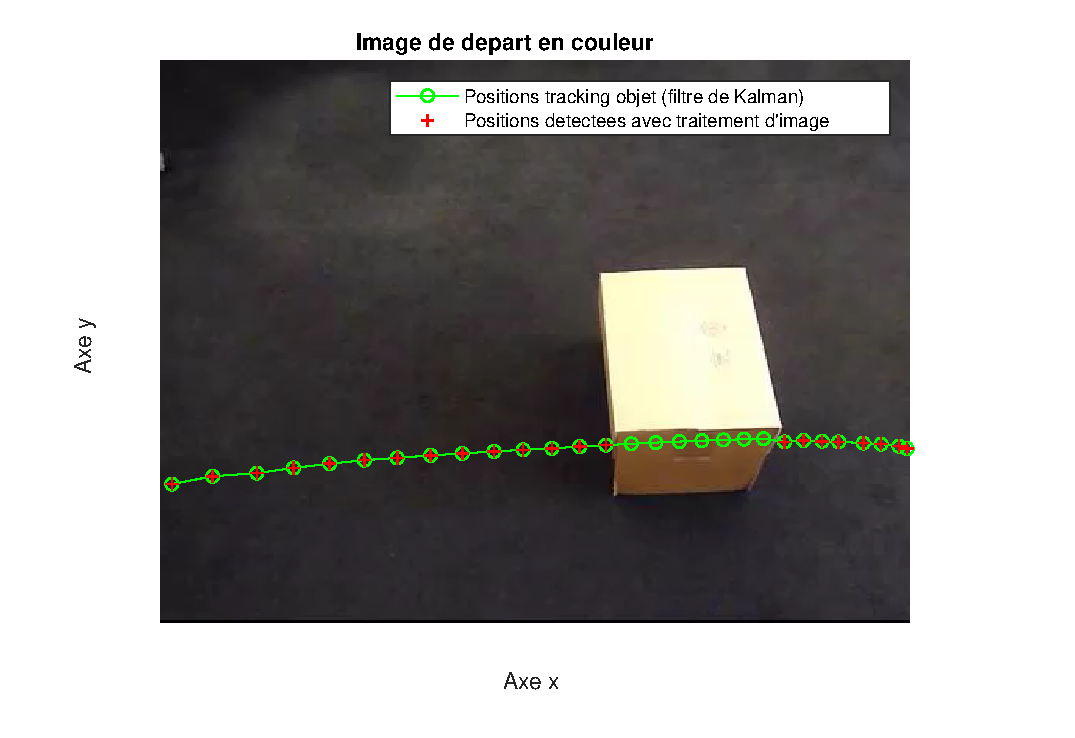
\includegraphics[width=20cm]{Images/Resultats/ImageDeDepartEnCourleur}}
\label{1}
\end{figure}

Sur la figure \ref{1}, les corrections des positions détectées semblent cohérentes. On remarque également que les prédictions des positions de la balle lorsqu'elle n'est pas détectée sont cohérentes.

\begin{figure}[H]
\caption{Positions successives de la balle}
\centerline{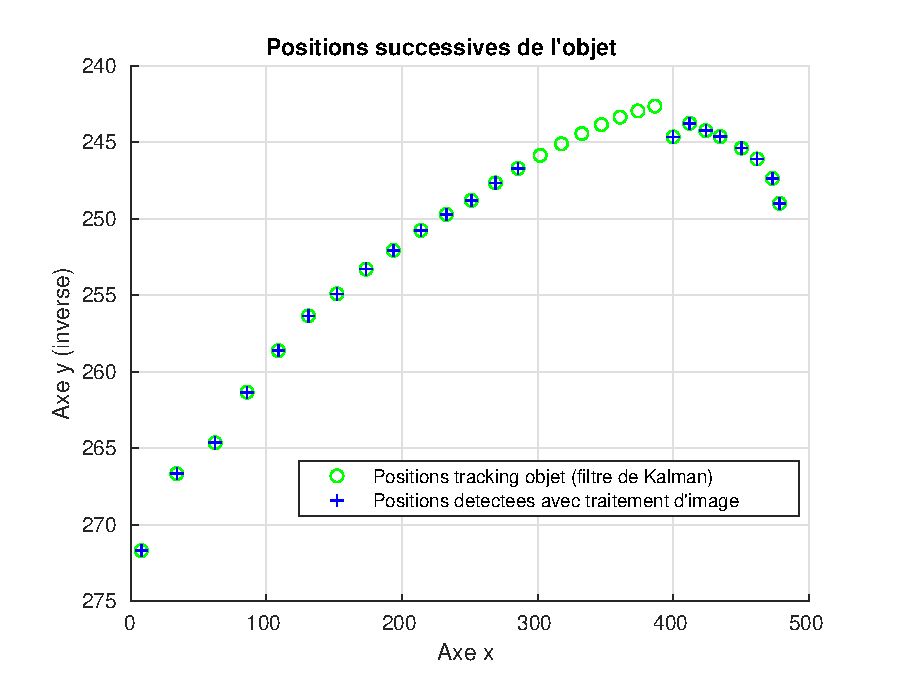
\includegraphics[width=20cm]{Images/Resultats/PositionsSuccessivesDeLObjet}}
\label{2}
\end{figure}

Sur la figure \ref{2}, on peut oberserver avec plus de détail les positions de la balle. On remarque que la prédiction des positions de la balle lorsqu'elle n'est pas détectée s'éloigne de sa vraie position. En effet, au bout de la septième prédiction, on voit que ce point est un peu éloigné de la position détectée lorsque la balle sort de l'autre côté de la boîte.

\subsection{Résultats avec $ dt = 1/30 \; s $ et ajustements de la vitesse et de l'accélération}

\begin{figure}[H]
\caption{Positions successives de la balle \--- Image 1 de la vidéo}
\centerline{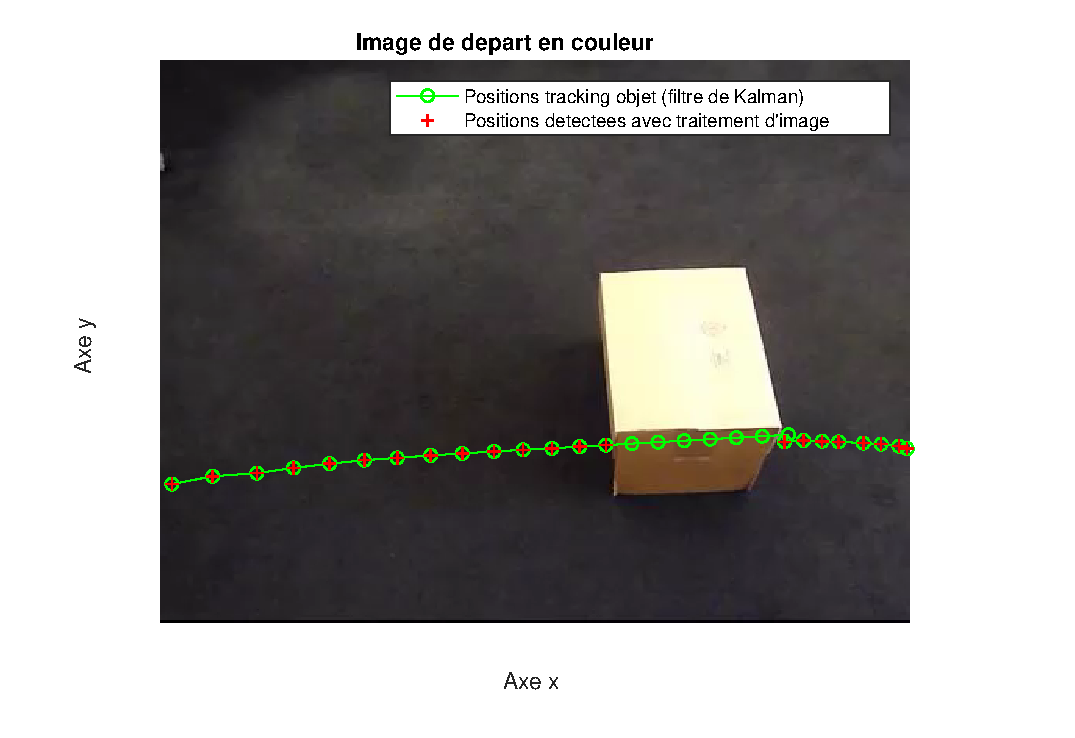
\includegraphics[width=20cm]{Images/Resultats/ImageDeDepartEnCourleur2}}
\label{3}
\end{figure}

Sur la figure \ref{3}, on remarque un problème lorsqu'on prédit la position de la balle quand elle n'est pas détectée. En effet, à la sortie de la boîte, le point prédit est trop loin.

\begin{figure}[H]
\caption{Positions successives de la balle}
\centerline{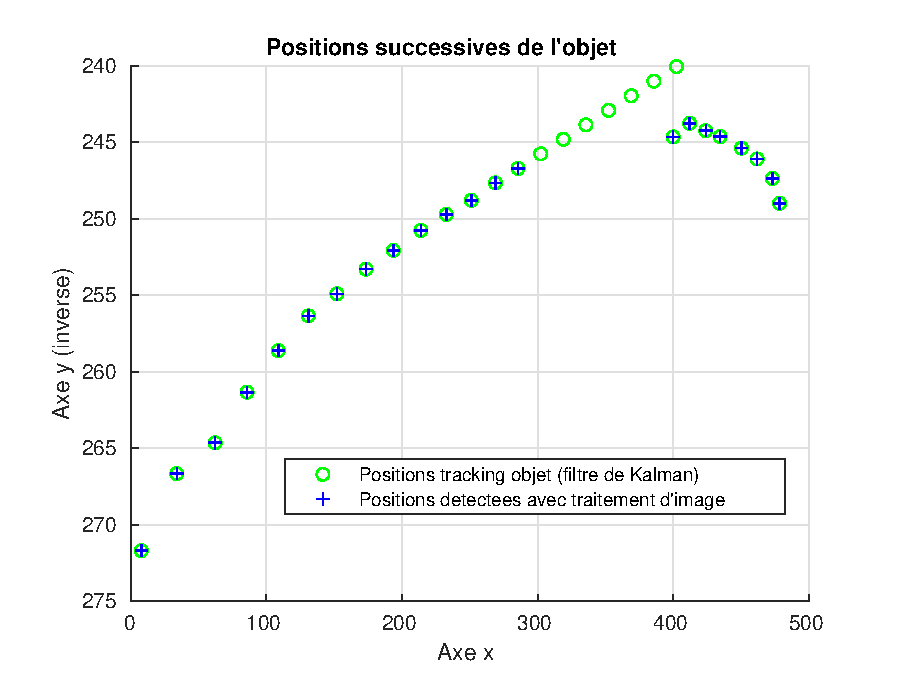
\includegraphics[width=20cm]{Images/Resultats/PositionsSuccessivesDeLObjet2}}
\label{4}
\end{figure}

Sur la figure \ref{4}, on remarque que les prédictions de la position de la balle quand elle n'est pas détectée ne sont pas bonnes. En effet, ces sept points ont une tendance linéaire et le septième point est éloigné du point détecté à la sortie de la boîte.




